\chapter{Grundlagen}
\label{cha:grundlagen}

% Abschnitt: Wartezeit Grundlagen
\section{Grundlagen der Bewertungen und Wartezeitenberechnung}
\label{sec:grundlagen:bewertugnen}

Da Freizeitparks mit sehr großen Besucherströmen zu tun haben, entstehen schnell lange Schlangen von Menschen an den verschiedensten Stellen, wie Attraktionen oder Essensausgaben, im Park. Die Zeit, die ein Besucher an einer Attraktion mit Warten verbringt, bezeichnet man als Wartezeit der Attraktion. Diese kann vom einstelligen bis hin zu einem dreistelligen Minutenbereich andauern. Größere Freizeitparks sind mittlerweile sehr gut darin, Besucherzahlen abzuschätzen und daraus aktuelle oder durchschnittliche Wartezeiten anzugeben. Diese werden meist am Eingang einer Attraktion angegeben.

%Bilder Wartemonitor
\begin{figure}[h]
    \centering
    \begin{minipage}{0.49\textwidth}
        \centering
        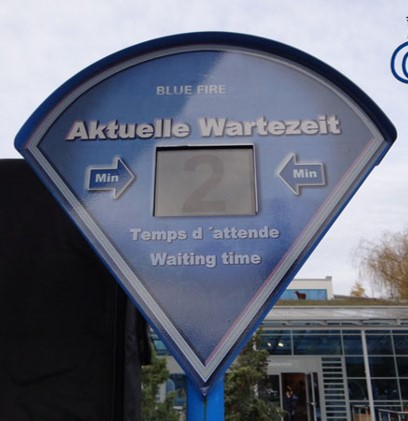
\includegraphics[width=0.4\textwidth]{img/motivation/wartezeit_2.jpg}
    \end{minipage}
    \begin{minipage}{0.49\textwidth}
        \centering
        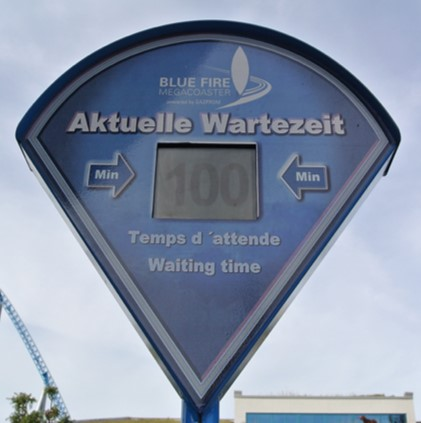
\includegraphics[width=0.4\textwidth]{img/motivation/wartezeit_100.jpg}
    \end{minipage}
\caption[Wartezeitanzeige im Park]{Wartezeitanzeige mit geringer (links) und hoher Wartezeit (rechts), TODO Bildquelle}
		\label{figure:grundlagenwaittime}
\end{figure}

Der Nachteil daran ist, dass die Wartezeiten  nur direkt beim Betreten der Attraktion sichtbar sind. Es wäre für den Besucher besser, diese auch andernorts und vergleichend betrachten zu können, um besser voraus planen zu können. Auch dafür haben einige Parks eine Lösung gefunden. So gibt es zum Beispiel Monitore mit allen Wartezeiten im Park oder eine parkeigene App mit allen aktuellen Wartezeiten. 

%Bilder Wartezeitübersicht
\begin{figure}[h]
    \centering
    \begin{minipage}{0.49\textwidth}
        \centering
        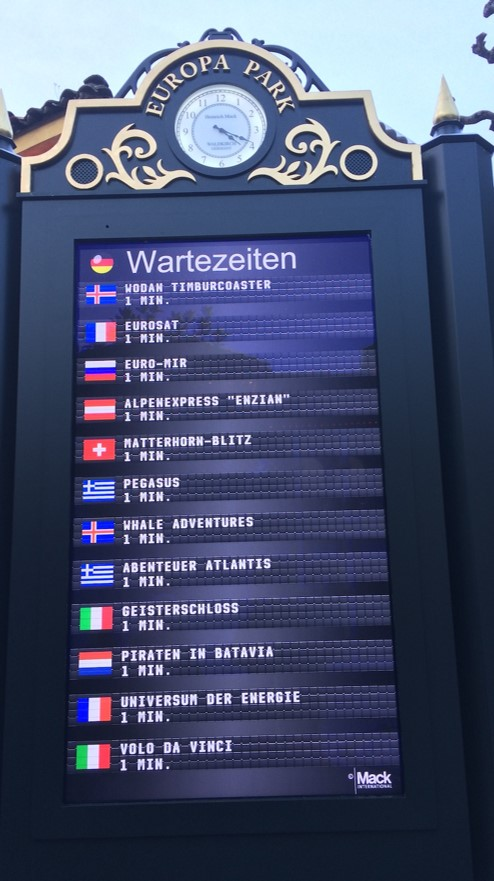
\includegraphics[width=0.4\textwidth]{img/motivation/wartezeit_anzeige.jpg}
    \end{minipage}
    \begin{minipage}{0.49\textwidth}
        \centering
        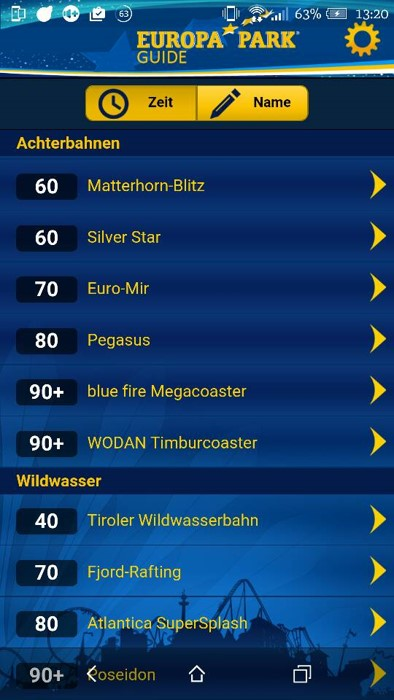
\includegraphics[width=0.4\textwidth]{img/motivation/app_official.jpg}
    \end{minipage}
\caption[Wartezeitübersicht im Europapark]{Wartezeitübersicht des Europaparks als Monitor (links) und als App (rechts), TODO Bildquelle}
		\label{figure:grundlagenwaittime2}
\end{figure}

Da diese parkeigenen Apps, aus verschiedenen Gründen, nur innerhalb des Parks funktionieren, bleibt auch hier das Problem, dass die aktuellen Wartezeiten nur innerhalb des Parks verfügbar sind und man nicht von außerhalb seinen Freizeitparkbesuch planen kann. Es kommt hinzu, dass man meistens nur eine aktuelle Wartezeit zur Verfügung hat, gerne aber weitere Informationen wie die Durchschnitte bestimmter Tage oder Uhrzeiten hätte. Außerdem gibt es bisher kein direktes Feedback der Nutzer über ihre tatsächlich verbrachte Wartezeit. 

Um all diese Probleme zu behben gibt es in unserer App verschiedene Metriken zum Vergleichen der Wartezeiten verschiedener Attraktionen. Diese werden nicht von den Freizeitparks zur Verfügung gestellt, sondern von den Nutzern selbst eingetragen, um somit aus der Gesamtheit aller Nutzerdaten verschiedene Werte berechnen zu können. Speziell unterscheidet unsere App zwischen folgenden fünf Arten von Wartezeiten einer Attraktion:
\begin{itemize}
\item Aktuelle Wartezeit: der Durchschnitt der neusten eingetragen Wartezeiten einer Attraktion, denkbar wäre hier auch das Einbinden von Livedaten aus vorhandenen APIs bestimmter Freizeitparks
\item Tagesdurchschnitt: der Durchschnitt aller eingetragenen Wartezeiten des aktuellen Tages einer Attraktion
\item Gesamtdurchschnitt: der Durchschnitt aller eingetragenen Wartezeiten einer Attraktion
\item Durchschnitt nach Uhrzeit: der Durchschnitt aller eingetragenen Wartezeiten einer Attraktion eines bestimmten Zeitraums
\item Wartezeitenliste: das Anzeigen aller eingetragenen Wartezeiten, welche nach Datum oder Dauer sortiert werden können
\end{itemize}

Da nicht nur die Wartezeit sondern auch die Qualität einer Attraktion ausschlaggebend ist, gibt es in unserer App zusätzlich ein Bewertungssystem für die einzelnen Attraktionen und auch für den Park insgesamt. Dieses ist wie jedes klassische Bewertungssystem durch das "5-Sterne-Bewertungssystem" realisiert. Dabei entsprechen 5 Sterne einer hervorragenden und 0 Sterne einer mangelhaften Bewertung.

% Abschnitt: Mobile Plattform
\section{Mobile Plattform Android}
\label{sec:grundlagen:plattforml}

Android ist ein mobiles Betriebssystem, also für Smartphones und Tablets, das von Google entwickelt wurde und auf Linux basiert. Die App-Entwicklung ist geprägt durch einzelne Aktivitäten (ein angezeigter Screen ist eine Aktivität), die miteinander kommunizieren und in ihrer 'Lebenszeit' ein vorgegebenes Zustandmodell \ref{figure:androidZustandsmodell} durchlaufen. Wir beschränken uns in Bezug auf die Plattform Android auf diese kurze Einführung, da die Plattform dank seiner weltweit hohen Verbreitung als bekannt angesehen werden dürfte.

\begin{figure}[htp]
	\centering
  	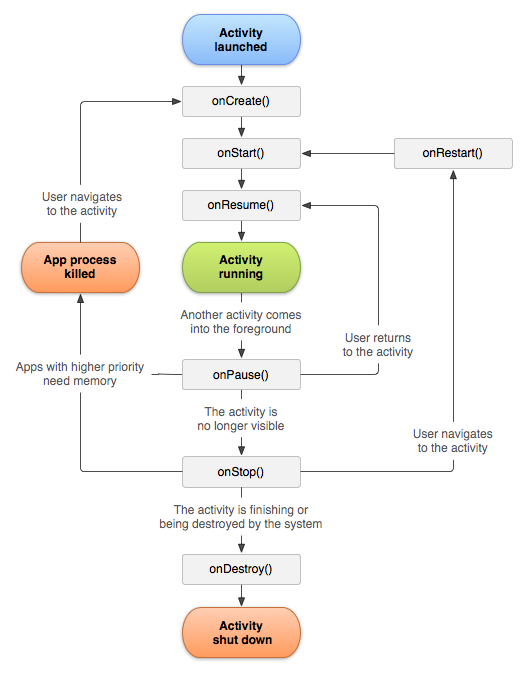
\includegraphics[width=0.5\textwidth]{img/modelle/AndroidZustandsmodell.png}
	\caption[Android Zustandsmodell]{Android Zustandsmodell, TODO Bildquelle}
	\label{figure:androidZustandsmodell}
\end{figure}

Dieses Zustandmodell ist auch anfangs einer der Nachteile von Android, da es nicht so leicht zu verstehen ist und uns auch ein paar Probleme bereitet hat. Nachdem wir uns aber im Laufe der App-Entwicklung immer mehr mit Android vertraut gemacht haben, war auch das Modell kein Problem mehr, sondern eher ein Vorteil, da es sehr logisch und durchdacht ist. Eine weitere Schwierigkeit, die während der Entwicklung aufgetreten ist, ist, dass es so viele verschiedene Android-Versionen und Geräte gibt. Da wir unsere App für so viele Versionen wie möglichen entwickeln wollten, kamen deshalb auch mal das ein oder andere Problem auf, wie z. B. dass manche Libraries oder Frameworks erst ab bestimmten Versionen verfügbar sind oder die vielen verschiedenen Geräte alle unterschiedlichen Seiten- und Größenverhältnisse haben.

Die Vorteile von Android überwiegen aber auf jeden Fall, vor allem, wenn man sich damit tiefer beschäftigt und eingearbeitet hat. Einer der größten Vorteile ist die sehr gute Dokumentation von Android durch die das Einlesen in die Möglichkeiten und Funktionen recht leicht ist. Auch die weltweite Verbreitung und Beliebtheit von Android ist hier ein Vorteil, da es sehr viele Entwickler gibt und so jedes Problem schon eimal aufgetreten ist und daher auch zu den allermeisten auch Lösungen oder Workarounds bekannt sind.
Außerdem wird Android stetig Weiterentwickelt, weshalb immer mehr möglich ist und der Umgang mit bestimmten Funktionen, wie z. B. der Zugriff auf Gerätefunktionen wie Kamera oder GPS immer leichter wird.
Weitere Vorteile für uns sind die Vertrautheit mit Java und die Einfachheit von Android Studio, welches wir für die Entwicklung unserer App benutzt haben.

% Abschnitt: Frameworks
\section{Frameworks}
\label{sec:grundlagen:frameworks}
Frameworks sind eine Art Gerüst oder Rahmen, die eingesetzt werden um das Programmieren zu vereinfachen und die geschriebenen Zeilen zu verringern.\\
Wir haben in unserer App die folgenden aufgelisteten Frameworks als Hilfen genutzt. Alle sind öffentlich und über den jeweiligen Namen auffindbar.
\begin{itemize}
\item Microsoft Azure Mobile App Service: Server mit persistenter Speicherung in SQLite-Datenbank (näheres dazu in Kapitel \ref{sec:implementierung:besonderheiten:azure})
\item Google Firebase: einfache Nutzerverwaltung (näheres dazu in Kapitel \ref{sec:implementierung:besonderheiten:firebase})
\item Cloudinary: kostenloses Hosten und Auslesen von Bildern via HTTP-Request
\item Picasso: erlaubt einfaches Handling (z. B. Größentransformationen) von Bildern in oftmals einer Zeile
\item Glide: ermöglicht eine bessere Darstellung der animierten Lade-Animation
\item MPAndroidCharts: ermöglicht die Erstellung von Diagrammen (in unserem Fall Säulendiagramme für die Statistiken)
\item MaterialChipsInput: Darstellung der Unterkategorien als Chips
\end{itemize}



















